\section{Marco Teórico} 
\subsection{Balanced Scorecard}
Es una herramienta revolucionaria para movilizar a la gente hacia el pleno cumplimiento de la misión, a través de canalizar las energías, habilidades y conocimientos específicos de la gente en la organización hacia el logro de metas estratégicas de largo plazo. 2El Balanced Scorecard (BSC) es por lo tanto un sistema de gestión estratégica de la empresa, que consiste en:

\begin{itemize}
\item Formular una estrategia consistente y transparente.  Comunicar la estrategia a través de la organización.
\item Coordinar los objetivos de las diversas unidades organizativas.
\item Conectar los objetivos con la planificación financiera y presupuestaria.
\item Identificar y coordinar las iniciativas estratégicas. 
\item Medir de un modo sistemático la realización, proponiendo acciones correctivas oportunas.
\end{itemize}



COMPONENTES BÁSICOS DE UN BSC:

\begin{itemize}
\item Cadena de Relaciones de Causa Efecto: Que expresen el conjunto de hipótesis de la estrategia a través de objetivos estratégicos y su logro mediante indicadores de desempeño.
\item Enlace a los Resultados Financieros: Los objetivos del negocio y sus respectivos indicadores, deben reflejar la composición sistémica de la estrategia, a través de cuatro perspectivas: Financiera, Clientes, Procesos Internos, y Aprendizaje y Crecimiento.
\item Balance de Indicadores de Resultados e Indicadores Guías: Se requiere un conjunto de indicadores que muestren las cosas que se necesita “hacer bien” para cumplir con el objetivo. Estos miden el progreso de las acciones. 
\item Mediciones que Generen e Impulsen el Cambio: La medición motiva determinados comportamientos, es importante definir indicadores que generen los comportamientos esperados, particularmente aquellos que orienten a la organización a la adaptabilidad ante un entorno en permanente y acelerado cambio.

\end{itemize}

PERSPECTIVAS DEL BALANCE SCORECARD \newline

\begin{itemize}
\item \textbf{Perspectiva Financiera} Su principal objetivo es responder a las expectativas de los accionistas. ¿Qué queremos cómo dueños o accionistas? Podría ser, ¿rentabilidad, crecimiento, valor agregado? Los resultados financieros se consiguen únicamente si los clientes están satisfechos. Es decir, la perspectiva financiera depende de cómo se construya la perspectiva del cliente ya que esta refleja el mercado en el cual se está compitiendo. 

\item \textbf{Perspectiva del Cliente} . Su principal objetivo es suministrar información importante para generar, adquirir, retener y satisfacer a los clientes, obtener cuota de mercado, rentabilidad, etc. ¿Cómo debemos satisfacer a nuestros clientes para alcanzar nuestros objetivos financieros? La satisfacción del cliente estará condicionada a la propuesta de valor que la organización o empresa les plantee. Esta propuesta de valor cubre básicamente, el espectro de expectativas compuesto por: Calidad, precio, relaciones, imagen.

\item \textbf{Perspectiva de Procesos Internos} En ella se identifican los objetivos e indicadores estratégicos asociados a los procesos clave de la organización o empresa, de cuyo éxito depende la satisfacción de las expectativas de clientes y accionistas. ¿Cuál debe ser el nivel de calidad y eficiencia de nuestros procesos para satisfacer las necesidades de los clientes? La perspectiva de procesos analiza la adecuación de los procesos internos (reducir los tiempos de manufactura, mejorar la calidad, ser más productivos) de la empresa de cara a la obtención de la satisfacción del cliente y logro de altos niveles de rendimiento financiero.

\item \textbf{Perspectiva de Aprendizaje Organizacional} En esta perspectiva se identifican la infraestructura necesaria para crear valor a largo plazo. Hay que lograr formación y crecimiento en 3 áreas: personas, sistemas y clima organizacional. Si la perspectiva de aprendizaje y crecimiento no identifica claramente qué tareas (capital humano), qué tecnología (capital de la información) y qué entorno (cultura organizacional) se necesitan para apoyar los procesos, la creación de valor no se producirá. Por lo tanto, tampoco se cumplirán los objetivos financieros.\newline
\end{itemize}

\begin{center}
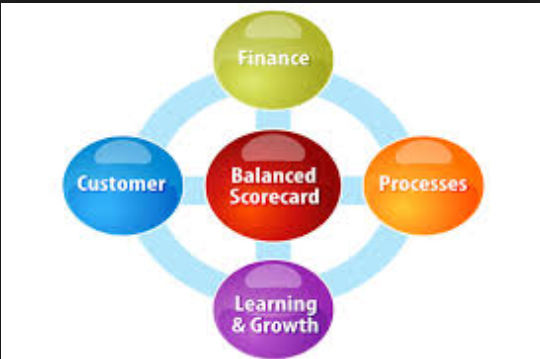
\includegraphics{images/BS/imagen.png}\newline
\end{center}

\subsection{Business Model Canvas}

La metodología de innovación y diseño incluye un Lienzo (Canvas) con 9 elementos que parten de determinar la Oferta de valor frente a la Segmentación de clientes de la empresa u organización. De ahí se clarifican los Canales de distribución y la Relaciones. Todos estos determinan los Beneficios e ingresos. Después se especifican los Recursos y las Actividades esenciales, que determinan los Costos más importantes. Finalmente se determinan las Alianzas necesarias para operar. La propuesta de trabajo es muy dinámica, con el trabajo de grupos interdisciplinares que combinan habilidades analíticas con pensamiento creativo a lo que Osterwalder llama “Pensamiento de diseño”. Se insta a los grupos a trabajar frente al lienzo pegado en la pared al tiempo que se representan en post-its las ideas con dibujos y un mínimo de palabras.\newline

\begin{center}
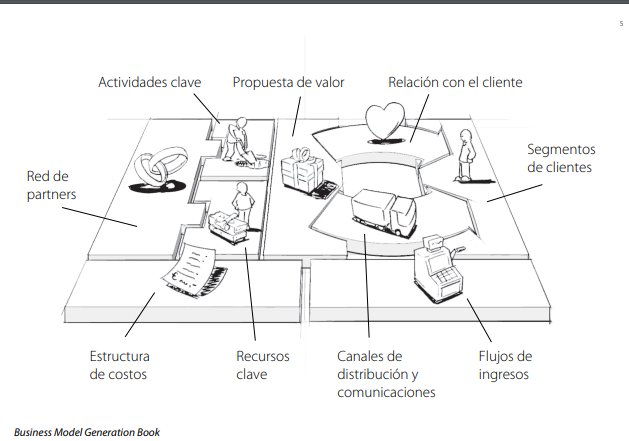
\includegraphics{images/BS/imagen2.png}\newline
\end{center}



PERSPECTIVAS DEL BALANCE SCORECARD \newline

\begin{itemize}
\item \textbf{Segmento de clientes} El objetivo es agrupar a nuestros clientes con características homogéneas en segmentos definidos y describir sus necesidades, averiguar información geográfica y demográfica, gustos, etc. Después, nos ocuparemos de ubicar a los clientes actuales en los diferentes segmentos para finalmente tener alguna estadística y crecimiento potencial de cada grupo. 

\item \textbf{Propuesta de Valor} El objetivo es de definir el valor creado para cada Segmento de clientes describiendo los productos y servicios que se ofrecen a cada uno. Para cada propuesta de valor hay que añadir el producto o servicio más importante y el nivel de servicio. Estas primeras dos partes son el núcleo del modelo de negocio.


\item \textbf{Canales de Distribución} Para cada producto o servicio que hemos identificado en el paso anterior hay que definir el canal de su distribución adecuado, añadiendo como información el ratio de éxito del canal y la eficiencia de su costo. 


\item \textbf{Relaciones con clientes} Aquí identificamos qué recursos de tiempo y monetarios utilizamos para mantenernos en contacto con nuestros clientes. Por lo general, si un producto o servicio tiene un costo alto entonces los clientes esperan tener una relación más cercana con nuestra empresa.  


\item \textbf{Flujos de ingresos} Este paso tiene como objetivo identificar que aportación monetaria hace cada grupo, y además de donde vienen las entradas (ventas, comisiones, licencias, etc.). Así po dremos tener una visión global de que grupos son más rentables y cuáles no. Aquí además de los beneficios económicos también habría que incluir si se obtienen otro tipo de beneficios sociales o medioambientales. 

\item \textbf{Recursos claves} Después de haber trabajado con los clientes, tenemos que centrarn os en la empresa, para ello debemos utilizar los datos obtenidos anteriormente, seleccionamos la propuesta de valor más importante y la relacionamos con el segmento de clientes, los canales de distribución, las relaciones con los clientes, y los flujos de ingreso para saber cuáles son los recursos clave que intervienen para que la empresa tenga la capacidad de entregar su oferta o propuesta de valor. Repetimos esta operación para cada propuesta de valor. 

\item \textbf{Actividades claves} Utilizando la propuesta de valor más importante, los canales de distribución y las relaciones con los clientes, definimos las actividades necesarias para entregar nuestra ofer ta. Repetimos esta operación para cada propuesta de valor.

\item \textbf{Red de Asociados, Alianzas y Colaboradores} En este apartado describimos a nuestros proveedores, socios, y asociado s con quienes trabajamos para que la empresa funcione. ¿Hasta qué punto son importantes? ¿Podemos reemplazarlos? ¿Se pueden convertir en competidores? 

\item \textbf{Costes económicos} Aquí especificamos los costos de la empresa empezando con el más alto (marketing, CRM, producción, salarios etc.). Luego relacionamos cada costo con los bloques definidos anteriormente, evitando generar demasiada complejidad. También se incluirán si existen los costes sociales y ambientales.

\end{itemize}


